\section{Code Structure}

\subsection{Hierarchy}

The \textbf{tools} folder contains the tools used to generate or import geometries and those used to exploit the simulation results :
\begin{itemize}
    \item \texttt{generateGeometry} : generates a geometry when given a shape (\textit{cube}, \textit{ellipsoid}), size, and parameters to create material spherical heterogeneity ({\tt nbr\_cavities, min\_radius, max\_radius}).
    \item \texttt{modifyGeometry} : modify an existing {\tt .stl} geometry to generate heteregenous cavities.
    \item \texttt{getThermalBarycenter} : returns the coordinates of the last point reaching a given temperature, as well as the time it occurs.
    \item \texttt{isosurface} : creates a 3D cooling animation over time with an isosurface at a given temperature. 
    \item \texttt{heatMapSlice} : creates a {\tt .pdf} file containing slice views of the diffusion. 
    \item \texttt{heatMapSliceAnimation} : creates a {\tt .avi} animation file with a slice view of the diffusion. 
    \item \texttt{geometryView} : creates a {\tt .pdf} file containing views of the geometry and mesh.
\end{itemize}

The \textbf{tools/utils} folder contains utilitaries useful to the \textbf{tools} folder functions : 
\begin{itemize}
    \item \texttt{digCube} : randomly creates spherical heterogeneity inside a cube.
    \item \texttt{digEllipsoid} : randomly creates spherical heterogeneity inside an ellipsoid.
    \item \texttt{spheresIntersect} : checks whether two spheres intersect.
\end{itemize}
\ 



\subsection{Variables}

The code mostly uses structure arrays to store geometry, material, options, and output data. \\

\subsubsection{Geometry}

A geometry structure is composed of the following mandatory fields : 

\renewcommand{\arraystretch}{1.5}
\begin{table}[h]
    \centering
    \begin{tabular}{|>{\customfont}c|>{\customfont}c|>{\customfont}c|}
        \hline 
        \rowcolor{gray!30}
        \textbf{Fields} & \textbf{Type} & \textbf{Description} \\ \hline
        \tt structure & \tt pde.DiscreteGeometry & Geometry \\ \hline 
        \tt exposed\_faces & \tt array (double) & ID of the faces exposed to the radiation flow \\ \hline 
        \tt nbr\_cavities\_faces	& \tt array (double) & Number of faces in all the cavities \\ \hline 
    \end{tabular}
\end{table}
\ 

\begin{minipage}{8.5cm}
\textsc{Matlab} counts the faces of the geometry in the following order :
\begin{enumerate}
    \item planar external faces
    \item curved/modified external faces
    \item faces inside the cavities
\end{enumerate} 

The following heterogeneous cube example is given. Here are the corresponding parameters : \\

{\tt exposed\_faces = [1:7]}\\
{\tt nbr\_cavities\_faces = 1}\\

\end{minipage}\hfill\begin{minipage}{7cm}
\begin{center}
    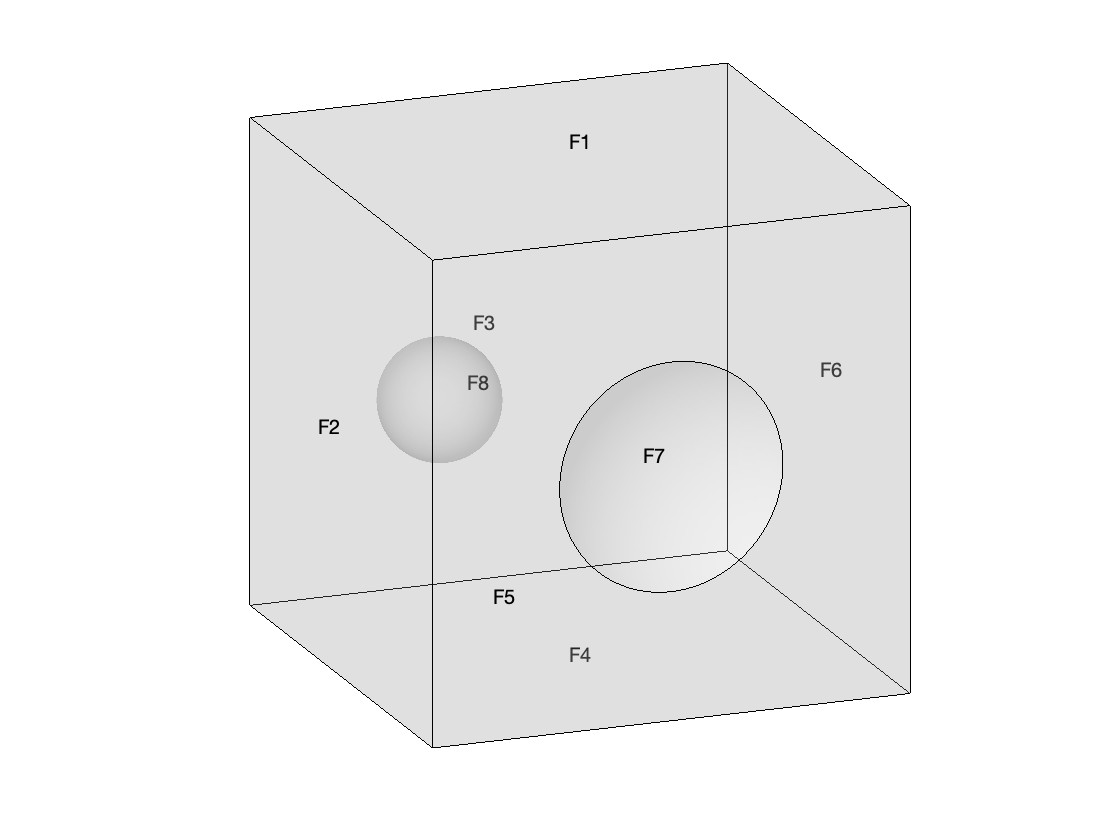
\includegraphics[scale=0.22]{ExampleFacesID.jpg}
\end{center}    
\end{minipage}
\ 


\subsubsection{Material}

A material structure is composed of the following mandatory fields :

\renewcommand{\arraystretch}{1.5}
\begin{table}[h]
    \centering
    \begin{tabular}{|>{\customfont}c|>{\customfont}c|>{\customfont}c|}
        \hline 
        \rowcolor{gray!30}
        \textbf{Fields} & \textbf{Type} & \textbf{Description} \\ \hline
        \tt rho & \tt array (double) & Density of the object ($kg \cdot m^3$) \\ \hline 
        \tt cp & \tt array (double) & Specific heat ($J  \cdot kg^{-1} \cdot K^{-1}$) \\ \hline 
        \tt T\_0	& \tt array (double) & Initial temperature of the object ($K$) \\ \hline 
        \tt lambda & \tt string & Thermal conductivity ($W m^{-1} K^{-1}$) \\ \hline
    \end{tabular}
\end{table}
\ 


\subsubsection{Options}

An options structure is composed of the following mandatory fields :

\renewcommand{\arraystretch}{1.5}
\begin{table}[h]
    \centering
    \begin{tabular}{|>{\customfont}c|>{\customfont}c|>{\customfont}c|}
        \hline 
        \rowcolor{gray!30}
        \textbf{Fields} & \textbf{Type} & \textbf{Description} \\ \hline
        \tt material & \tt material & The properties of the material composing the main geometry\\ \hline 
        \tt cavities\_material & \tt material & The properties of the material composing the cavities \\ \hline 
        \tt T\_out	& \tt array (double) & Temperature outside the object $(K)$ \\ \hline 
        \tt eps & \tt array (double) & Emissivity of the object (no dimension) \\ \hline 
        \tt dt & \tt array (double) & Simulation time step $(s)$ \\ \hline 
        \tt tmax & \tt array (double) & Duration of the simulation $(s)$ \\ \hline
    \end{tabular}
\end{table}
\ 

\subsubsection{Output}

\renewcommand{\arraystretch}{1.5}
\begin{table}[h]
    \centering
    \begin{tabular}{|>{\customfont}c|>{\customfont}c|>{\customfont}c|}
        \hline 
        \rowcolor{gray!30}
        \textbf{Fields} & \textbf{Type} & \textbf{Description} \\ \hline
        \tt Temperature & \tt array (double) & Temperature values at nodes\\ \hline 
        \tt SolutionTimes & \tt array (double) & Solution times \\ \hline 
        \tt XGradients	& \tt array (double) & x-component of the temperature gradient at nodes\\ \hline 
        \tt YGradients & \tt array (double) & y-component of the temperature gradient at nodes\\ \hline 
        \tt ZGradients & \tt array (double) & z-component of the temperature gradient at nodes \\ \hline 
        \tt Mesh & \tt FEMesh & Finite element mesh \\ \hline
    \end{tabular}
\end{table}
\ 
